\documentclass{IEEEtran}

\usepackage{graphicx}
\usepackage{amsthm}
\usepackage{amssymb}
\usepackage{amsmath}
\usepackage{algorithm}
\usepackage{algorithmicx}
\usepackage{algpseudocode}
\usepackage{booktabs}
\usepackage{color}

\newcommand{\comment}[1]{}

%\renewcommand{\baselinestretch}{0.95}
%\setlength{\textfloatsep}{0.1cm}
%\setlength{\abovecaptionskip}{0.1cm}

\begin{document}

\title{Preserving Differential Privacy on Ranked Similarity Search over Encrypted Cloud Data}
\author{
Shiyu Ji}
\maketitle

\newtheorem{definition}{Definition}
\theoremstyle{definition}
\newtheorem{theorem}{Theorem}
\theoremstyle{plain}
\newtheorem{lemma}{Lemma}
\theoremstyle{plain}
\newtheorem{corollary}{Corollary}
\theoremstyle{plain}

\section{Problem Formulation}
\subsection{The System and Threat Model}

\begin{figure}
\centering
\includegraphics[width=0.45\textwidth]{system_model.eps}
\caption{The architecture of ranked similarity search over encrypted cloud data.}
\label{fig:system_model}
\end{figure}

As in Fig. \ref{fig:system_model}, we consider a cloud data hosting service which consists of three entities: the data owner, the data users and the semi-trusted cloud data server. The data owner has a collection of documents that need to be outsourced to the semi-trusted cloud server. The outsourced documents must be encrypted since the data owner does not want to reveal the documents to the semi-trusted server. The encryption scheme will be given later. On the other hand, the data users want to search over the encrypted documents. To enable this, the data owner prepares a search index of the outsourced documents, and then uploads the encrypted index to the server. On a similarity search request, an authorized data user firstly gets the corresponding trapdoors and keys from the data owner, and uses the keys to encrypt the query, and then sends the encrypted search query to the cloud server. Upon receiving the search query, the server should securely search on the index and return the top $k$ most similar documents in the encrypted form to the user.

We assume the cloud server is \emph{semi-trusted}, or \emph{honest-but-curious}, i.e., the server will honestly do as described above, but it also wants to know any information of the outsourced documents and the submitted search queries. We consider the \emph{Ciphertext-Only Attack}, in which the server only has the submitted encrypted documents and queries, but it initially has no knowledge about their plaintext. We will also consider another stronger attack, in which we assume the server has some knowledge about the outsourced content, e.g., the frequency distribution. Thus some statistical attacks may be launched.

\subsection{Our Goals}
We want to design an efficient and secure ranked search scheme over encrypted cloud data that satisfy the requirements above, and we also want it to keep privacy to some extent.

\textbf{Efficiency}. The algorithms should be efficient, e.g., 1) encryption over the documents, index and queries, 2) search over the encrypted index, etc.

\textbf{Dynamic updating support}. The data owner should be able to update the documents and index efficiently at any time.

\textbf{Confidentiality}. The content of the documents, the entries in the index and the submitted queries should not be revealed to the cloud server.

\textbf{Privacy preserving}. We want to prevent the cloud server from learning anything about the outsourced documents, index or queries submitted by users. We will investigate the cases as follows:
\begin{itemize}
\item \textbf{Query unlinkability}. The server should be difficult to tell whether two encrypted queries are from the same search request (e.g., the same keywords or terms) if these two queries are generated by similar search requests. Note the server can easily tell apart the queries from very different requests, since the returned top $k$ documents could be very different.
\item \textbf{Keyword privacy}. The server should not know any information about the keywords or terms in the search request.
\end{itemize}

\subsection{Notations and Preliminaries}
\begin{itemize}
\item $\mathbf{F}$ \---- The collection of the documents to be outsourced: $\mathbf{F} = \{f_1, f_2, \cdots, f_n\}$ where $f_i$ denotes the $i$-th document.
\item $\mathbf{C}$ \---- The collection of the encrypted documents in $\mathbf{F}$: $\mathbf{C} = \{c_1, c_2, \cdots, c_n\}$ where each $c_i$ is the encrypted form of $f_i$.
\item $I$ \---- The index built for $\mathbf{C}$: $I = \{I_1, I_2, \cdots, I_n\}$. Denote by $I_i$ the entry of $c_i$. Each $I_i$ is a vector determined by the keywords and terms in $f_i$.
\item $q$ \---- The query vector determined by the keywords and terms in the search request.
\item $\hat{f}$ \---- The top $k$ documents: $\hat{f} = \{\hat{f}_1, \hat{f}_2, \cdots, \hat{f}_k\}$ with the highest similarities to the query $q$.
\end{itemize}
\emph{Cosine similarity} is a popular measure to evaluate the similarity between two vectors in information retrieval \cite{ATY13,TAJY14}. Given a set of vectors $v_i = (v_{i,1}, v_{i,2}, \cdots, v_{i,m})^T$ where each vector is normalized to a unit length, and has at most $m$ features (if $v_i$ does not have feature $k$, we can set $v_{i,k}$ to be zero), the cosine similarity between vectors is defined as follows:
$$Sim(v_i,v_j) = \sum_{k=1}^m v_{i,k}\cdot v_{j,k}.$$
Note that the cosine similarity of two vectors equals to their dot product. We say two vectors are similar if their cosine similarity exceeds some threshold $\tau$. For a ranked search over the documents $\mathbf{F}$, given the query vector $q$, we want the cloud server to return the top $k$ documents $\{\hat{f}_i\}$ with the highest cosine similarities $Sim(\hat{f}_i, q)$.


\bibliographystyle{./IEEEtran}
\bibliography{./sim_privacy}
\end{document}
